\chapter{METODOLOGIA CIENTÍFICA}

\section{Classificação da pesquisa}

Este trabalho caracteriza-se como uma pesquisa aplicada, de abordagem quantitativa e com caráter experimental. Segundo \citeonline{gil_2002}, pesquisas podem estar associadas a razões de ordem prática, relacionadas à produção de conhecimento com vistas à sua aplicação. Nesse sentido, este trabalho possui natureza aplicada por utilizar conceitos e ferramentas de simulação computacional para investigar um problema relacionado ao tráfego urbano. O objetivo não é desenvolver uma nova ferramenta de simulação, mas utilizar uma ferramenta existente como apoio para analisar como diferentes comportamentos de motoristas podem influenciar o desempenho do tráfego em um cenário urbano simulado.

A abordagem quantitativa se justifica pelo uso de métricas numéricas para comparar os resultados obtidos nas simulações. Entre essas métricas, poderão ser considerados o tempo médio de viagem, a velocidade média, o tempo parado, a formação de filas e a vazão de veículos. Esses dados permitirão comparar os cenários simulados de forma objetiva, observando diferenças entre configurações de fluxo e perfis de motoristas.

A pesquisa também possui caráter experimental, pois serão criados cenários controlados de simulação nos quais determinadas variáveis serão alteradas. Segundo \citeonline{gil_2002}, a pesquisa experimental envolve a seleção de variáveis capazes de influenciar o objeto de estudo e a definição de formas de controle e observação de seus efeitos. Neste trabalho, as principais variáveis estarão relacionadas ao fluxo de veículos e aos parâmetros de comportamento dos motoristas. Ao manter uma mesma rede viária e modificar esses fatores, será possível observar como cada configuração interfere no desempenho geral do tráfego.

É importante destacar que o trabalho não pretende reproduzir com precisão absoluta o trânsito real da região estudada. A proposta é construir um cenário simplificado, baseado em um recorte urbano real, que permita realizar comparações entre diferentes condições de simulação. Dessa forma, o foco da pesquisa está na análise dos efeitos produzidos pelos perfis de motoristas, e não na validação completa do funcionamento do trânsito da cidade.

Assim, a metodologia será organizada em etapas que envolvem a escolha da área de estudo, a construção do cenário de simulação, a definição dos perfis de motoristas, a configuração dos cenários, a execução das simulações e a análise dos resultados obtidos. Essas etapas serão detalhadas nas seções seguintes.

\section{Área de estudo}

O cenário de simulação será baseado em um recorte da região central do município de Videira, em Santa Catarina, com foco no entorno da Praça Nereu Ramos e em vias adjacentes. A escolha dessa região considera sua configuração viária, que envolve conversões, mudanças de direção, aproximações entre vias e diferentes possibilidades de deslocamento dos veículos.

Embora a região apresente uma dinâmica de circulação em torno de um ponto central, ela não será tratada neste trabalho como uma rotatória formal. O trecho será considerado como uma área urbana com organização viária própria, na qual diferentes fluxos se encontram e os motoristas precisam tomar decisões relacionadas à escolha de faixa, entrada no fluxo, conversões e continuidade do deslocamento. Essa característica torna o cenário adequado para observar como diferentes perfis de motoristas podem influenciar o desempenho do tráfego.

O recorte escolhido não será limitado apenas ao entorno imediato da Praça Nereu Ramos. Também serão considerados trechos próximos de entrada e saída, de modo que os veículos possam ser inseridos na rede antes de chegarem à região central da simulação e possam deixar o cenário após atravessá-la. Essa escolha busca evitar uma representação artificial, na qual os veículos surgem diretamente no ponto analisado, sem formar um fluxo de tráfego minimamente coerente.

A proposta não é reproduzir todos os detalhes físicos e operacionais da região real, mas construir uma representação simplificada e funcional do trecho urbano escolhido. Dessa forma, elementos que não estiverem diretamente relacionados ao objetivo do trabalho poderão ser simplificados ou desconsiderados, desde que a estrutura principal da circulação seja mantida. O foco estará na criação de um cenário que permita comparar, de forma controlada, os efeitos de diferentes perfis de motoristas sobre o desempenho do tráfego.

A Figura~\ref{fig:cenario-estudo} apresenta uma representação preliminar da área de estudo considerada para a construção do cenário de simulação.

\begin{figure}[H]
    \centering
    \captionstyle[\centering]{\centering}
    \caption{Representação preliminar da área de estudo no SUMO}
    \label{fig:cenario-estudo}

    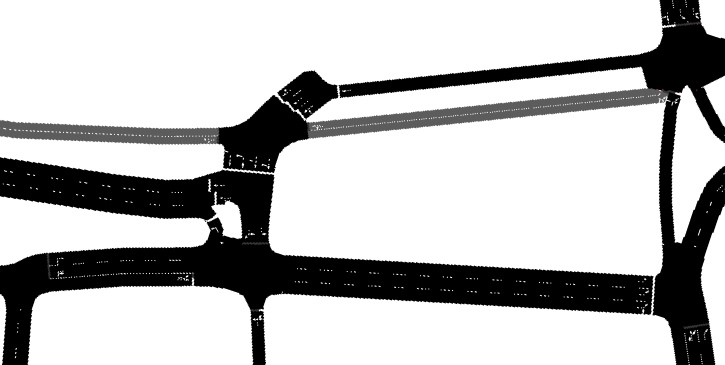
\includegraphics[width=0.70\textwidth]{images/cenario_estudo_sumo.png}

    \par\vspace{0.25cm}
    \begin{minipage}{0.70\textwidth}
        \footnotesize Fonte: Elaborado pelo autor.
    \end{minipage}
\end{figure}

\section{Ferramentas utilizadas}

Para o desenvolvimento deste trabalho, será utilizado o \gls{sumo}, do inglês \textit{Simulation of Urban MObility}, como ferramenta principal para a construção e execução das simulações microscópicas de tráfego. A ferramenta foi escolhida por ser \textit{open source}, permitir a representação individual dos veículos, possibilitar a configuração de parâmetros de condução e gerar arquivos de saída úteis para a análise dos resultados.

A rede viária inicial será baseada em dados do OpenStreetMap. Para sua preparação serão utilizados recursos do próprio \gls{sumo}, como o \textit{netconvert}, responsável pela conversão da rede para o formato do simulador, e o \textit{NetEdit}, utilizado para visualizar e editar vias, conexões, sentidos de circulação e permissões de conversão.

Também poderão ser utilizados \textit{scripts} em Python para auxiliar na automação das simulações, na alteração de parâmetros, na organização dos arquivos de saída e no tratamento dos dados obtidos. O ambiente previsto para o desenvolvimento desses \textit{scripts} será o Visual Studio Code. Para a análise dos resultados, poderão ser utilizadas bibliotecas Python voltadas ao tratamento de dados e geração de gráficos, como \textit{pandas} e \textit{matplotlib}.

\section{Construção do cenário de simulação}

A construção do cenário de simulação será realizada a partir do recorte urbano definido para o trabalho. Inicialmente, a rede viária será importada com base em dados do OpenStreetMap e convertida para o formato do \gls{sumo}. Essa rede será utilizada como ponto de partida para a modelagem do cenário.

Após a importação, a rede será analisada no \gls{sumo} e no \textit{NetEdit}. Essa etapa será necessária para verificar se a estrutura obtida está adequada às necessidades do cenário de simulação. Serão observados principalmente os sentidos das vias, as conexões entre os trechos, as permissões de conversão, a quantidade de faixas e os pontos de entrada e saída de veículos.

Caso sejam identificadas inconsistências, serão realizados ajustes manuais na rede. Esses ajustes serão importantes especialmente no entorno da Praça Nereu Ramos, pois a região possui diferentes possibilidades de deslocamento, mudanças de direção e aproximações entre fluxos. O objetivo será obter uma representação simplificada, mas funcional, da circulação no trecho analisado.

Também poderão ser feitas simplificações no cenário, removendo ou desconsiderando elementos que não contribuam diretamente para os objetivos do trabalho. Essa escolha busca manter o escopo viável, concentrando a análise nos trechos que influenciam a circulação principal da área estudada.

Depois da construção da rede, serão feitos testes preliminares no \gls{sumo} para verificar a coerência operacional do cenário. Nessa etapa, serão observados aspectos como continuidade das rotas, ausência de bloqueios indevidos, funcionamento das conexões entre vias, comportamento dos veículos nos pontos de entrada e saída e formação de filas decorrente da própria configuração simulada. Caso sejam identificados problemas, a rede será ajustada novamente até que esteja adequada para a configuração dos fluxos, perfis de motoristas e cenários de simulação.

\section{Definição dos perfis de motoristas}

Para analisar o impacto do comportamento dos condutores no tráfego urbano, serão definidos perfis de motoristas a serem utilizados nas simulações. Esses perfis serão representados por meio de parâmetros computacionais do \gls{sumo} relacionados à forma de condução dos veículos.

Inicialmente, serão considerados três perfis principais: cauteloso, normal e agressivo. O perfil cauteloso representará uma configuração com tendências mais conservadoras de condução, como maior distância de seguimento e menor aceitação de lacunas. O perfil normal será utilizado como referência intermediária, sem características extremas de condução. Já o perfil agressivo representará uma configuração com tendências opostas, como menor distância de seguimento, maior aceleração e maior aceitação de lacunas.

A definição desses perfis não tem como objetivo classificar todos os motoristas reais de forma definitiva. Trata-se de uma simplificação necessária para permitir a comparação entre cenários simulados. Dessa forma, os perfis serão utilizados como abstrações computacionais, permitindo observar como diferentes parâmetros de condução podem influenciar o desempenho do tráfego.

Entre os parâmetros que poderão ser utilizados para diferenciar os perfis estão aceleração, desaceleração, distância mínima de seguimento, velocidade desejada, tempo de reação ou seguimento e aceitação de lacunas. O Quadro~\ref{qua:perfis-motoristas} apresenta a tendência esperada desses parâmetros para cada perfil. Os valores concretos desses parâmetros não serão definidos de forma arbitrária. Na etapa de desenvolvimento do TCC, eles serão estabelecidos a partir da literatura relacionada à heterogeneidade de motoristas, dos parâmetros configuráveis disponíveis no \gls{sumo}, da documentação da ferramenta e de testes preliminares no cenário construído. A literatura será utilizada para orientar as tendências esperadas de cada perfil, como diferenças na distância de seguimento, na aceleração, na desaceleração e no tempo de reação dos motoristas \cite{ossen_2011,zhai_2021,mecheva_2022,makridis_2023}. Esses testes não terão como objetivo realizar uma calibração completa com dados reais de tráfego, mas verificar se os valores adotados produzem comportamentos coerentes para fins comparativos, sem gerar situações artificiais, como bloqueios indevidos, acelerações incompatíveis ou instabilidade na circulação. Os valores finais utilizados em cada perfil serão documentados no TCC, permitindo a reprodução dos cenários simulados.


\begin{quadro}[htbp]
\centering
\caption{Tendências esperadas dos parâmetros por perfil de motorista}
\label{qua:perfis-motoristas}
\small
\renewcommand{\arraystretch}{1.25}

\begin{tabular}{|p{5.4cm} | p{3.0cm} | p{2.8cm} | p{2.8cm}|}
\hline
\textbf{Parâmetro} & \textbf{Cauteloso} & \textbf{Normal} & \textbf{Agressivo} \\
\hline
Aceleração & Menor & Intermediária & Maior \\
\hline
Desaceleração & Mais conservadora & Intermediária & Mais intensa \\
\hline
Distância mínima de seguimento & Maior & Intermediária & Menor \\
\hline
Velocidade desejada & Menor & Intermediária & Maior \\
\hline
Tempo de reação ou seguimento & Maior & Intermediário & Menor \\
\hline
Aceitação de lacunas & Menor & Intermediária & Maior \\
\hline
\end{tabular}

\par\vspace{0.25cm}
\begin{minipage}{\textwidth}
\footnotesize Fonte: Elaborado pelo autor.
\end{minipage}

\end{quadro}

\section{Definição dos cenários de simulação}

Os cenários de simulação serão definidos a partir da combinação entre a rede viária construída, os níveis de fluxo de veículos e as composições dos perfis de motoristas configurados. A intenção é realizar comparações controladas, permitindo variar separadamente a intensidade do fluxo e a participação dos diferentes perfis de condução.

Inicialmente, serão considerados três níveis de fluxo: baixo, médio e alto. Esses níveis não terão como objetivo reproduzir exatamente a quantidade real de veículos da região estudada, mas representar diferentes condições de carregamento da rede. Os valores associados a cada nível serão definidos durante os testes preliminares, considerando o comportamento do cenário no \gls{sumo}.

Também serão consideradas diferentes composições dos perfis cauteloso, normal e agressivo. Além de cenários de referência compostos apenas por motoristas com perfil normal, serão avaliadas composições mistas, incluindo situações com distribuição mais equilibrada entre os perfis e situações com maior participação de determinado perfil. Os percentuais finais serão definidos após testes preliminares, buscando produzir diferenças suficientes para comparação sem criar configurações excessivamente artificiais.

Os cenários serão organizados de forma que seja possível comparar diferentes composições mantendo o mesmo nível de fluxo e, de forma complementar, comparar diferentes níveis de fluxo mantendo a mesma composição de perfis. Essa organização busca permitir uma análise mais clara dos efeitos associados ao comportamento dos motoristas e das alterações decorrentes do carregamento da rede.

\begin{quadro}[H]
\centering
\caption{Estrutura inicial dos cenários de simulação}
\label{qua:cenarios-simulacao}
\small
\renewcommand{\arraystretch}{1.25}

\begin{tabular}{|p{4.7cm}| p{3cm}| p{7.2cm}|}
\hline
\textbf{Tipo de cenário} & \textbf{Fluxo previsto} & \textbf{Composição prevista} \\
\hline
Referência & Baixo, médio e alto & Motoristas com perfil normal. \\
\hline
Composição mista equilibrada & Baixo, médio e alto & Participação semelhante dos perfis cauteloso, normal e agressivo. \\
\hline
Predominância cautelosa & Baixo, médio e alto & Maior participação de motoristas com perfil cauteloso. \\
\hline
Predominância agressiva & Baixo, médio e alto & Maior participação de motoristas com perfil agressivo. \\
\hline
\end{tabular}

\par\vspace{0.25cm}
\begin{minipage}{\textwidth}
\footnotesize Fonte: Elaborado pelo autor.
\end{minipage}

\end{quadro}

O Quadro~\ref{qua:cenarios-simulacao} apresenta a estrutura inicial prevista para os experimentos. As proporções dos perfis e os valores correspondentes aos níveis de fluxo ainda serão definidos durante a etapa prática do trabalho. Os testes preliminares serão utilizados para verificar quais configurações produzem condições adequadas para a comparação entre os cenários.

A execução dessas combinações permitirá observar tanto os efeitos associados à composição dos perfis de motoristas quanto as possíveis mudanças desses efeitos em diferentes condições de carregamento da rede. As configurações finais utilizadas nos experimentos serão documentadas no TCC para permitir a reprodução das simulações.

\section{Métricas de avaliação}

A avaliação dos cenários simulados será realizada por meio de métricas relacionadas ao desempenho do tráfego. Essas métricas serão obtidas a partir dos arquivos de saída gerados pelo \gls{sumo} após a execução das simulações. A escolha das métricas busca permitir a comparação entre os diferentes cenários e níveis de fluxo definidos no trabalho.

Entre as principais métricas previstas estão o tempo médio de viagem, a velocidade média, o tempo parado, a formação de filas e a vazão de veículos. O tempo médio de viagem será utilizado para observar quanto tempo, em média, os veículos levam para percorrer o cenário. A velocidade média permitirá avaliar a fluidez do tráfego, enquanto o tempo parado indicará situações em que os veículos permanecem retidos ou com deslocamento interrompido.

A formação de filas será considerada para identificar pontos de maior retenção no cenário, principalmente em trechos de aproximação, conversão ou entrada no fluxo. Já a vazão de veículos será utilizada para observar a quantidade de veículos que consegue atravessar ou concluir o percurso no período simulado. Essas métricas, analisadas em conjunto, permitirão avaliar as diferenças de desempenho do tráfego entre os cenários simulados.

Caso necessário, outras métricas disponibilizadas pelo \gls{sumo} poderão ser consideradas durante a etapa prática do trabalho, desde que estejam relacionadas aos objetivos da pesquisa. A definição final das métricas dependerá da viabilidade de extração dos dados e da relevância de cada informação para a comparação entre os cenários simulados.

\section{Procedimentos de análise dos resultados}

Após a execução das simulações, os dados gerados pelo \gls{sumo} serão organizados para permitir a comparação entre os cenários definidos. Essa etapa envolverá a leitura dos arquivos de saída, a seleção das métricas de interesse e a organização dos resultados em tabelas ou gráficos, de acordo com a necessidade da análise.

As comparações serão realizadas considerando tanto as diferentes composições de perfis de motoristas quanto os níveis de fluxo de veículos. Para analisar os efeitos associados aos perfis de condução, serão comparados cenários com diferentes composições mantendo o mesmo nível de fluxo. De forma complementar, cenários com a mesma composição serão comparados em diferentes níveis de fluxo, permitindo observar como o carregamento da rede pode influenciar os resultados.

Os cenários de referência, compostos por motoristas com perfil normal, serão utilizados como base para parte das comparações. A análise buscará identificar diferenças no tempo médio de viagem, na velocidade média, no tempo parado, na formação de filas e na vazão, considerando também se os efeitos das diferentes composições se tornam mais perceptíveis conforme aumenta a intensidade do fluxo.

Para reduzir a influência de variações ocasionais, serão realizadas múltiplas execuções de cada configuração utilizando diferentes sementes pseudoaleatórias definidas e registradas. Dessa forma, será possível considerar a variabilidade introduzida pelos elementos aleatórios da simulação e, ao mesmo tempo, manter um registro que permita reproduzir posteriormente as execuções realizadas. A quantidade de repetições será estabelecida após os testes preliminares, considerando a variabilidade e a estabilidade observadas nos resultados.

Os resultados das diferentes execuções poderão ser consolidados por meio de valores médios e outras formas de organização que se mostrarem adequadas durante a análise. A necessidade de procedimentos estatísticos adicionais será avaliada posteriormente, de acordo com as características e a variabilidade dos dados obtidos.

Por fim, os resultados serão discutidos com base nos objetivos definidos no trabalho. A análise buscará identificar como diferentes composições de perfis de motoristas influenciam o desempenho do tráfego urbano no cenário simulado e como esses efeitos se relacionam com os diferentes níveis de carregamento da rede.

\section{Limitações do estudo}

Este trabalho não tem como objetivo reproduzir com precisão absoluta o trânsito real da região estudada. A proposta é construir um cenário urbano simplificado, baseado em um recorte real, que permita comparar de forma controlada os efeitos de diferentes composições de perfis de motoristas no desempenho do tráfego.

Alguns fatores presentes no trânsito real poderão ser desconsiderados ou simplificados, como comportamento de pedestres, transporte coletivo, estacionamento, condições climáticas, acidentes, obras e variações reais de demanda ao longo do dia. Essas simplificações são necessárias para manter o escopo do trabalho compatível com os objetivos da pesquisa e com o tempo disponível para seu desenvolvimento.

\begin{figure}[htbp]
    \centering
    \captionstyle[\centering]{\centering}
    \caption{Etapas previstas para o desenvolvimento da pesquisa}
    \label{fig:fluxograma-metodologia}

    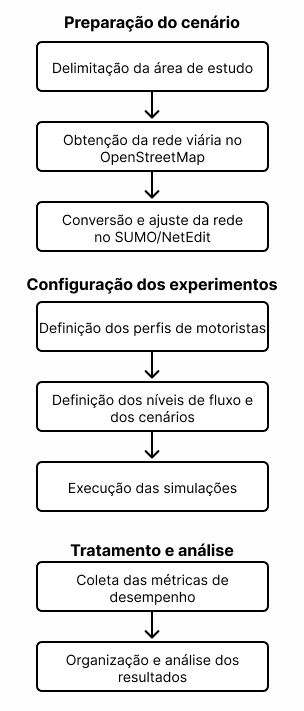
\includegraphics[width=0.32\textwidth]{images/fluxograma_metodologia.png}

    \par\vspace{0.15cm}
    \begin{minipage}{0.32\textwidth}
        \footnotesize Fonte: Elaborado pelo autor.
    \end{minipage}
\end{figure}

Dessa forma, os resultados obtidos deverão ser interpretados como uma análise comparativa entre cenários simulados, e não como uma previsão exata do funcionamento do trânsito da região. O foco estará na observação dos efeitos produzidos pelas diferentes composições de perfis de motoristas e pelos níveis de fluxo definidos para a simulação. A Figura~\ref{fig:fluxograma-metodologia} apresenta, de forma resumida, as etapas previstas para a execução da pesquisa.